\documentclass{article}

\newcommand{\dir}{~/projects/latex}
\input{\dir/include.tex}
\load{full}
\setLang{de}

\setup{Theoretische Informatik}

\newcommand{\hdelta}{\hat{\delta}}

\begin{document}
\startDocument
\usetcolorboxes

\vspace{2cm}
\begin{Huge}
    \begin{center}
        TITLE PAGE COMING SOON
    \end{center}
\end{Huge}


\vspace{4cm}
\begin{center}
    \begin{Large}
        ``\textit{A funny quote from the lecture still needed}``
    \end{Large}

    \hspace{3cm} - A professor in TI, 2025
\end{center}

\vspace{3cm}
\begin{center}
    HS2025, ETHZ\\[0.2cm]
    \begin{Large}
        Summary of the book \color{MidnightBlue}\fbox{\href{https://link.springer.com/book/10.1007/978-3-658-06433-4}{Theoretische Informatik}}\color{black}
    \end{Large}\\[0.2cm]
    by Prof. Dr. Juraj Hromkovic
\end{center}

\newpage

\printtoc{Orange}

\begin{scriptsize}
    \begin{itemize}
        \item \textit{Note: Definitions, Lemmas, etc are often 1:1 copies from the book or paraphrased (as I did not find an easier way of stating them)}
        \item \textit{Note: In case I forgot to add the PDF page numbers, you can take the PDF page number is given by $P_{\text{PDF}} = P_{\text{Book}} + 15$}
    \end{itemize}
\end{scriptsize}

\newpage


% Combinatorics
\newsection
\section{Combinatorics}
\subsection{Introduction}
Combinatorics was developed from the willingness of humans to gamble and the fact that everybody wanted to win as much money as possible.

\subsection{Simple counting operations}
The easiest way to find the best chance of winning is to write down all possible outcomes. This can be very tedious though when the list gets longer.

We can note this all down as a list or as a tree diagram. So-called Venn Diagrams might also help represent the relationship between two sets or events. Essentially a Venn Diagram is a graphical representation of set operations such as $A \cup B$.


\subsection{Basic rules of counting}
\subsubsection{Multiplication rule}
If one has $n$ possibilities for a first choice and $m$ possibilities for a second choice, then there are a total of $n \cdot m$ possible combinations.

When we think about a task, and we have an \textbf{and} in between e.g. properties, we need to multiply all the options.

\subsubsection{Addition rule}
If two events are mutually exclusive, the first has $n$ possibilities and the second one has $m$ possibilities, then both events together have $n+m$ possibilities.

When we think about a task, and we have an \textbf{or} in between e.g. properties, then we need to add all the options.


\newpage
\subsection{Factorial}
\begin{definition}[]{Factorial}
    The factorial stands for the product of the first $n$ natural numbers where $n \ge 1$. Notation: $!$
    \[
        n! = n \cdot (n - 1) \cdot (n - 2) \cdot \ldots \cdot 3 \cdot 2 \cdot 1
    \]
    Additionally, $0! = 1$. We read $n!$ as ``\textit{n factorial}''
\end{definition}

\subsubsection{Operations}
We can rewrite $n!$ as $n \cdot (n - 1)!$ or $n \cdot (n - 1) \cdot (n - 2)!$ and so on.

It is also possible to write $7 \cdot 6 \cdot 5$ with factorial notation: $\displaystyle \frac{7!}{4!}$, or in other words, for any excerpt of a factorial sequence: \[n \cdot (n - 1) \cdot \ldots \cdot m = \frac{n!}{(m - 1)!}\]


\subsection{Permutations}
\begin{definition}[]{Permutations}
    A permutation of a group is any possible arrangement of the group's elements in a particular order\\

    \textbf{Permutation rule without repetition:} The number of $n$ \textbf{\textit{distinguishable}} elements is defined as: $n!$
\end{definition}


\subsubsection{Permutation with repetition}
For $n$ elements $n_1,n_2,\ldots,n_k$ of which some are identical, the number of permutations can be calculated as follows:
\[
    p = \frac{n!}{n_1! \cdot n_2! \cdot \ldots \cdot n_k!}
\]
where $n_k$ is the number of times a certain element occurs. 
As a matter of fact, this rule also applies to permutations without repetition, as each element occurs only once, which means the denominator is $1$, hence $\displaystyle \frac{n!}{(1!)^n} = n!$

\inlineex \smallhspace CANADA has $6$ letters, of which $3$ letters are the same. So the word consists of $3$ A's, which can be arranged in $3!$ different ways, a C, N and D, which can be arranged in $1!$ ways each. Therefore, we have:
\[
    \frac{6!}{3!\cdot 1! \cdot 1! \cdot 1!} = \frac{6!}{3!} = 6 \cdot 5 \cdot 4 = 120
\]

Since $1!$ equals $1$, we can always ignore all elements that occur only once, as they won't influence the final result.


\newpage
\subsection{Variations}
\begin{definition}[]{Variations}
    A \textbf{\textit{variation}} is a selection of $k$ elements from a universal set that consists of $n$ \textit{distinguishable} elements.\\

    \textbf{Variation rule without repetition:} The $_n\mbox{P}_k$ function is used to \textit{\textbf{place}} $n$ elements on $k$ places. In a more mathematical definition:
    The number of different variations consisting of $k$ different elements selected from $n$ distinguishable elements can be calculated as follows:

    \[
        \frac{n!}{(n - k)!} = _n\mbox{P}_k
    \]
\end{definition}

\subsubsection{Variations with repetition}
If an element can be selected more than once and the order matters, the number of different variations consisting of $k$ elements selected from $n$ distinguishable elements can be calculated using $n^k$



\subsection{Combinations}
\begin{definition}[]{Combination}
    A combination is a selection of $k$ elements from $n$ elements in total without any regard to order or arrangement.

    \textbf{Combination rule without repetition:} \[
        _n\mbox{C}_k = {n\choose k} = \frac{_n\mbox{P}_k}{k!} = \frac{n!}{(n - k)! \cdot k!}
    \]
\end{definition}

\subsubsection{Combination with repetition}
In general the question to ask for combinations is, in how many ways can I distribute $k$ objects among $n$ elements?
\[
    _{n + k - 1}\mbox{C}_k = {n + k - 1\choose k} = \frac{(n + k - 1)!}{k!(n - 1)!}
\]



\subsection{Binomial Expansion}
\label{sec:binomial-expansion}
Binomial expansion is usually quite hard, but it can be much easier than it first seems. The first term of the expression of $(a + b)^n$ is always $1 a^n b^0$. Using the formula for combination without repetition, we can find the coefficients of each element:

\begin{center}
    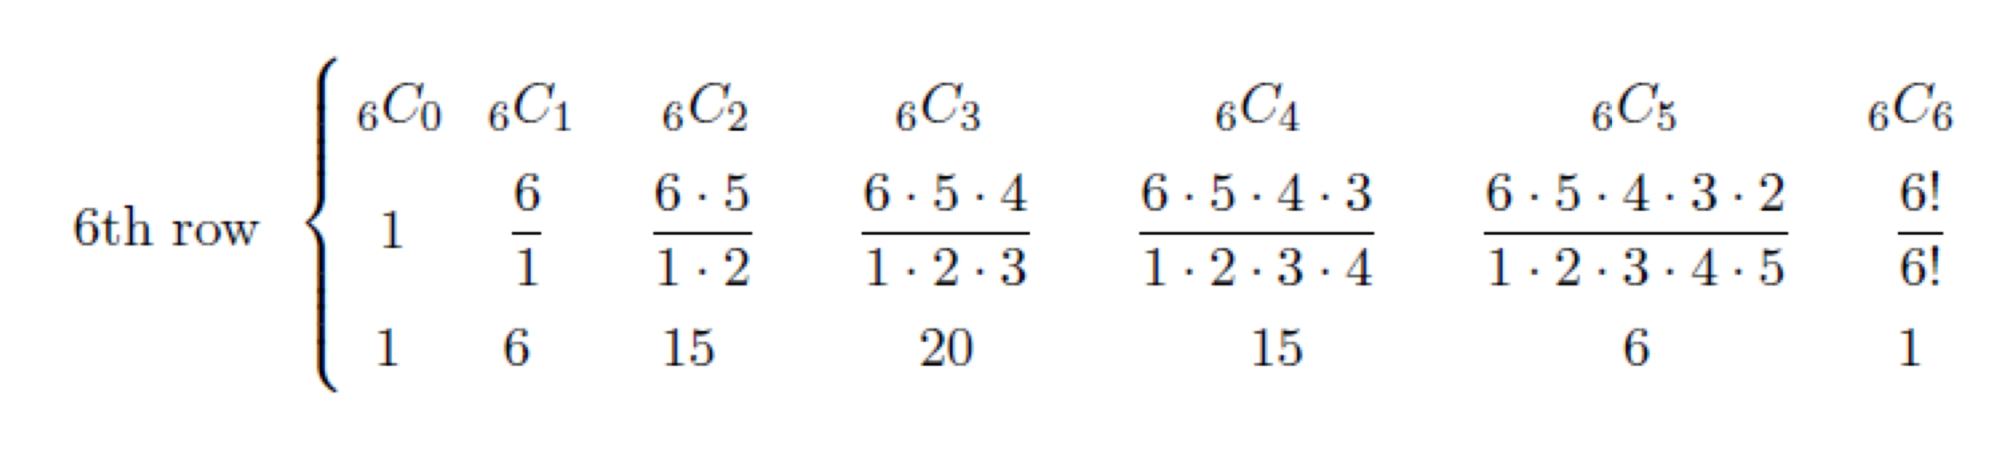
\includegraphics[width=0.6\linewidth]{./assets/binomialExpansion.png}
\end{center}

This theory is based on the Pascal's Triangle and the numbers of row $n$ correspond to the coefficients of each element of the expanded term.

We can calculate the coefficient of each part of the expanded term $k$ with combinatorics as follows: $\displaystyle {n\choose k}$

\begin{formula}[]{Binomial Expansion}
    \textbf{\textit{\underbar{In general:}}}
    \[
        (a + b)^n = 1a^nb^0 + {n\choose 1} a^{n-1}b^{1} + {n\choose 2} a^{n-2}b^{2} + \ldots + {n\choose n - 1} a^{1}b^{n - 1} + {n\choose n} a^{0}b^{n}
    \]
\end{formula}


\subsection{Overview}
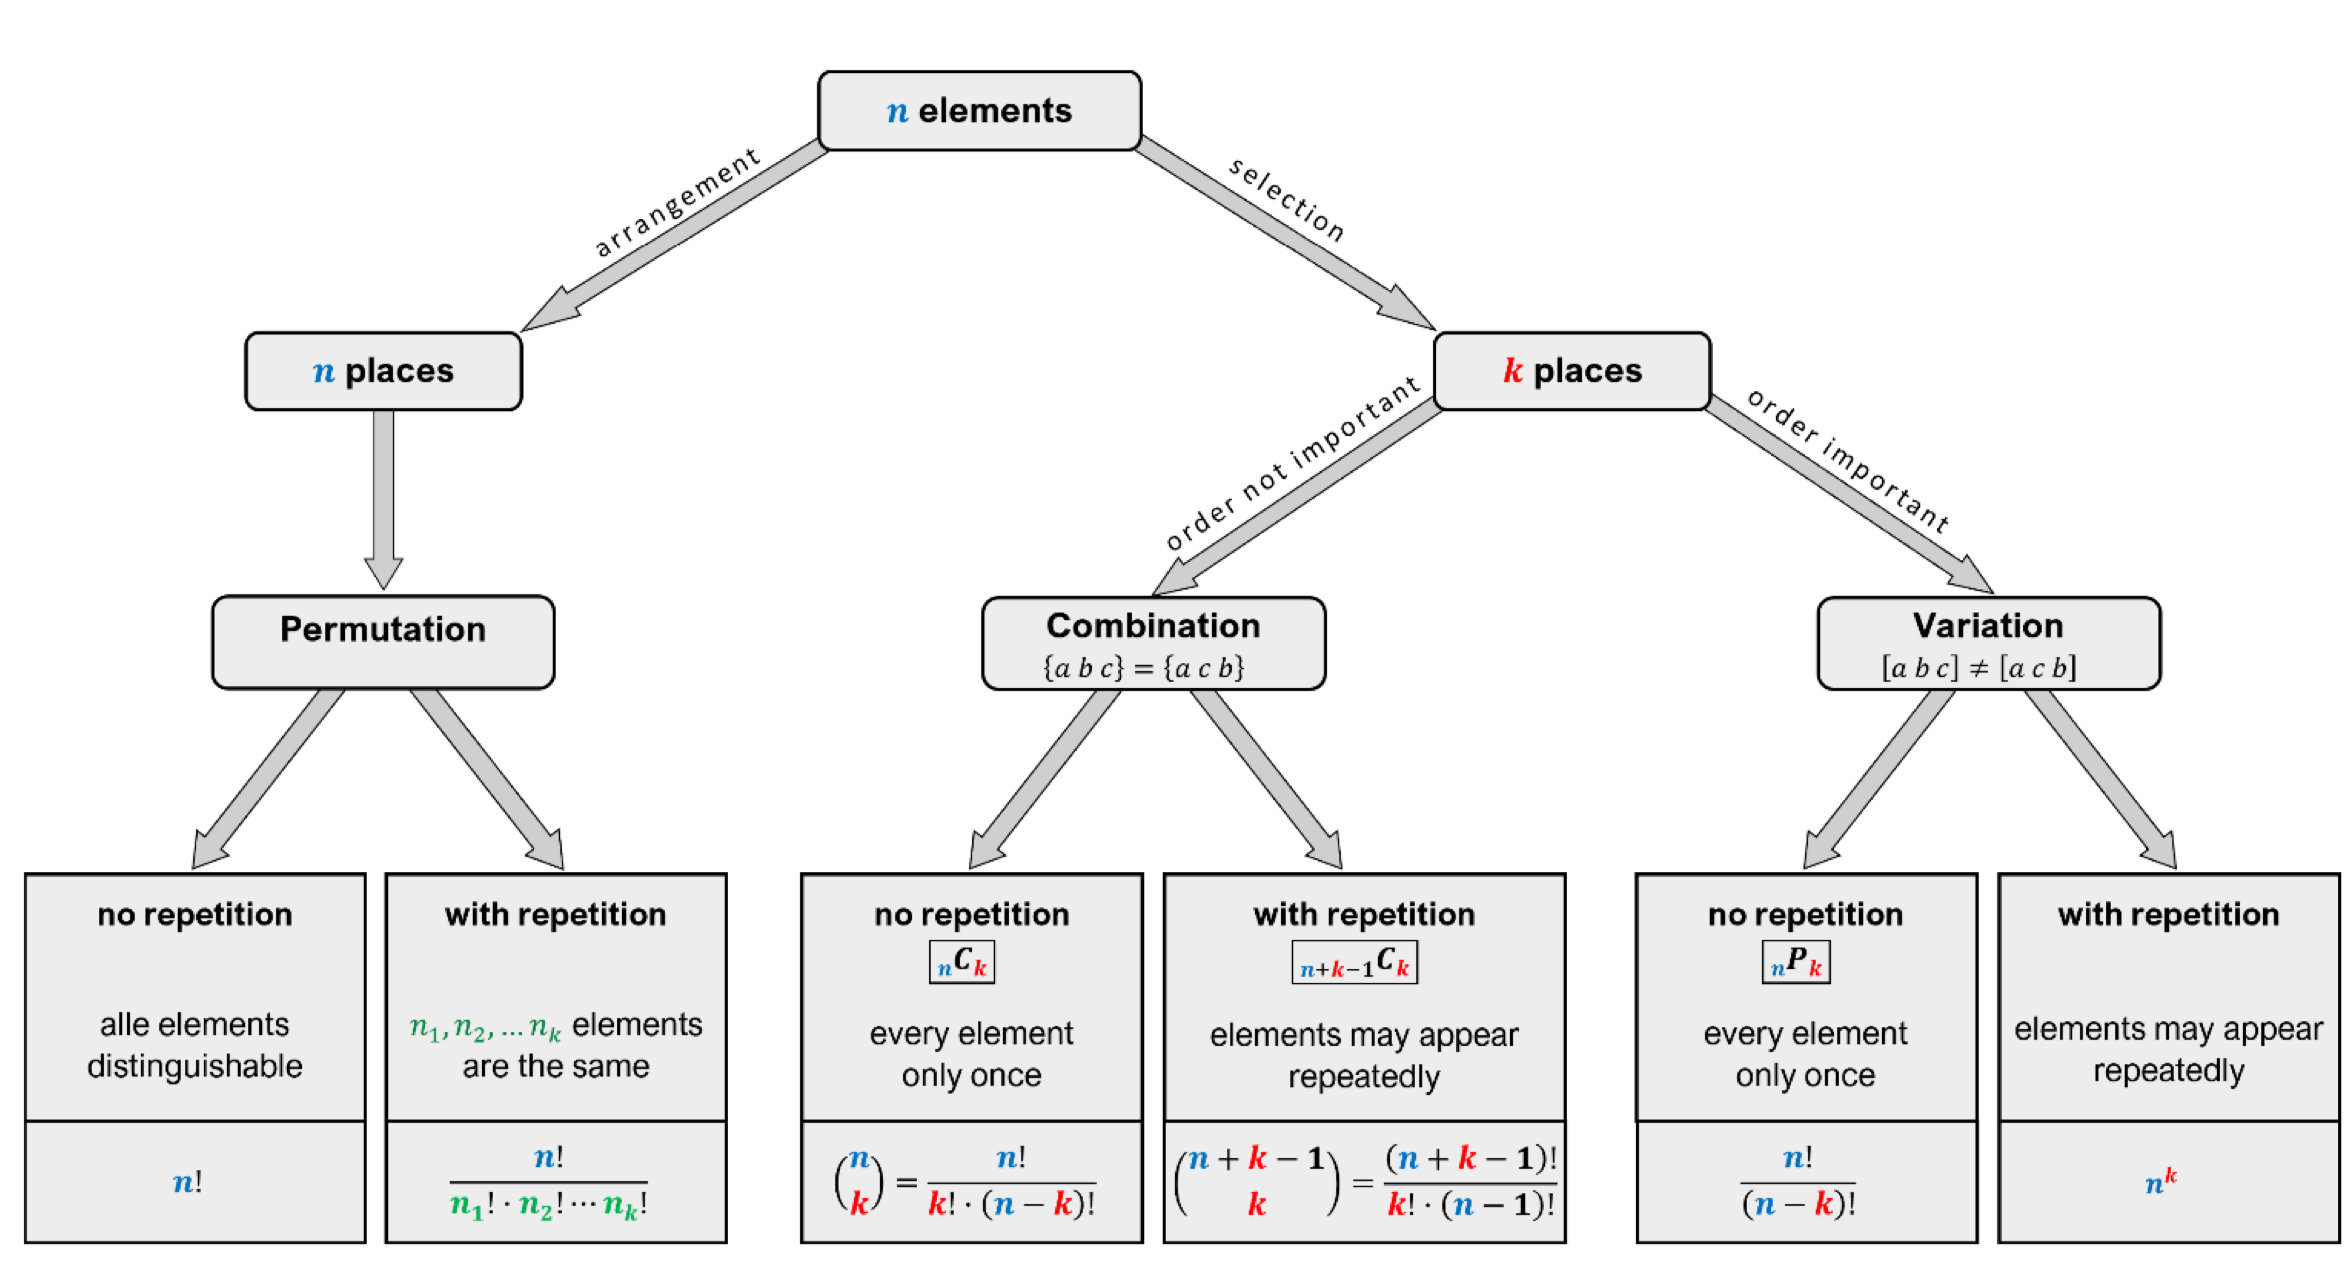
\includegraphics[width=1\linewidth]{./assets/overview.png}



% ┌                                                ┐
% │                   Alphabets                    │
% └                                                ┘
\newsection
\section{Alphabete, Wörter, Sprachen und Darstellung von Problemen}
\stepcounter{subsection}
\subsection{Alphabete, Wörter, Sprachen}

\begin{definition}[]{Alphabet}
    Eine endliche, nicht leere Menge $\Sigma$. Elemente sind Buchstaben (Zeichen \& Symbole). 

    Beispiele: $\alphabets{bool}$, $\alphabets{lat}$ latin characters, $\alphabets{Tastatur}$, $\Sigma_m$ $m$-adische Zahlen ($m$-ary numbers, zero index)
\end{definition}

\begin{definition}[]{Wort}
    Über $\Sigma$ eine (möglicherweise leere) Folge von Buchstaben aus $\Sigma$. Leeres Wort $\lambda$ (ab und zu $\varepsilon$) hat keine Buchstaben.

    $|w|$ ist die Länge des Wortes (Anzahl Buchstaben im Wort), während $\Sigma^*$ die Menge aller Wörter über $\Sigma$ ist und $\Sigma^+ = \Sigma^* - \{\lambda\}$

    In diesem Kurs werden Wörter ohne Komma geschrieben, also $x_1x_2\ldots x_n$ statt $x_1, x_2, \ldots, x_n$.
    Für das Leersymbol gilt $|\text{\textvisiblespace}|$, also ist es nicht dasselbe wie $\lambda$
\end{definition}

Für viele der Berechnungen in Verbindung mit der Länge der Wörter kann Kombinatorik nützlich werden. 
In Kapitel \ref{sec:combinatorics} findet sich eine Zusammenfassung über jenes Thema (in English)

Ein mögliches Alphabet beispielsweise um einen Graphen darzustellen ist folgendes: 

Angenommen, wir speichern den Graphen als Adjezenzmatrix ab, dann können wir beispielsweise mit dem Alphabet $\Sigma = \{0, 1, \#\}$ diese Matrix darstellen, in dem wir jede neue Linie mit einem $\#$ abgrenzen.
Das Problem hierbei ist jedoch, dass dies nicht so effizient ist, besonders nicht, wenn der Graph sparse ist, da wir dann viele \# im Vergleich zu nützlicher Information haben.

\begin{definition}[]{Konkatenation}
    $\Sigma^* \times \Sigma^* \rightarrow \Sigma^*$, so dass Kon$(x, y) = x \cdot y = xy \smallhspace \forall x, y \in \Sigma^*$.

    Intuitiv ist dies genau das was man denkt: Wörter zusammenhängen (wie in Programmiersprachen). 
    Die Operation ist assoziativ und hat das Neutralelement $\lambda$, was heisst, dass $(\Sigma^*, \text{Kon})$ ein Monoid ist.

    Offensichtlich ist die Konkatenation nur für ein-elementige Alphabete kommutativ.

    Die Notation $(abc)^n$ wird für die $n$-fache Konkatenation von $abc$ verwendet
\end{definition}


\begin{definition}[]{Umkehrung}
    Sei $a = a_1 a_2 \ldots a_n$, wobei $a_i \in \Sigma$ für $i \in \{1, 2, \ldots, n\}$, dann ist die Umkehrung von $a$, $a^\tR = a_n a_{n - 1} \ldots a_1$
\end{definition}


\begin{definition}[]{Iteration}
    Die $i$-te Iteration $x^i$ von $x \in \Sigma^*$ für alle $i \in \N$ ist definiert als $x^0 = \lambda$, $x^1 = x$ und $x^i = xx^{i - 1}$
\end{definition}


\begin{definition}[]{Teilwort, Präfix, Suffix}
    Seien $v, w \in \Sigma^*$
    \begin{itemize}
        \item $v$ heisst \bi{Präfix} von $w \Longleftrightarrow \exists y \in \Sigma^* : w = vy$
        \item $v$ heisst \bi{Suffix} von $w \Longleftrightarrow \exists x \in \Sigma^* : w = xv$
        \item $v$ heisst \bi{Teilwort} von $w \Longleftrightarrow \exists x, y \in \Sigma^* : w = xvy$
        \item $v \neq \lambda$ heisst \bi{echtes} Teilwort (gilt auch für Präfix, Suffix) von $w$ genau dann, wenn $v \neq w$ und $v$ ein Teilwort (oder eben Präfix oder Suffix) von $w$ ist
    \end{itemize}
\end{definition}

\begin{definition}[]{Kardinalität, Vorkommen und Potenzmenge}
    Für Wort $x \in \Sigma^*$ und Buchstabe $a \in \Sigma$ ist $|x|_a$ definiert als die Anzahl Male, die $a$ in $x$ vorkommt.

    Für jede Menge $A$ ist $|A|$ die Kardinalität und $\mathcal{P}(A) = \{S | S \subseteq A\}$ die Potenzmenge von $A$
\end{definition}


\begin{definition}[]{Kanonische Ordnung}
    Wir definieren eine Ordnung $s_1 < \ldots < s_m$ auf $\Sigma$. Die \bi{kanonische Ordnung} auf $\Sigma^*$ für $u, v \in \Sigma^*$ ist definiert als:
    \begin{align*}
        u < v \Longleftrightarrow |u| < |v| \lor (|u| = |v| \land u = x \cdot s_i \cdot u' \land v = x \cdot s_j \cdot v') \text{ für beliebige $x, u', v' \in \Sigma^*$ und $i < j$}
    \end{align*}

    Oder in Worten, geordnet nach Länge und dann danach für den ersten nicht gemeinsamen Buchstaben, nach dessen Ordnung.
\end{definition}


\begin{definition}[]{Sprache}
    $L \subseteq \Sigma^*$ ist eine Sprache, deren Komplement $L^C = \Sigma^* - L$ ist. 
    Dabei ist $L_{\emptyset}$ die \bi{leere Sprache} und $L_{\lambda}$ die einelementige Sprache die nur aus dem leeren Wort besteht.

    Die \bi{Konkatenation} von $L_1$ und $L_2$ ist $L_1 \cdot L_2 = L_1 L_2 = \{ vw \divides v \in L_1 \land w \in L_2 \}$ und $L^0 := L_{\lambda}$ und $L^{i + 1} = L^i \cdot L \smallhspace \forall i \in \N$ und $L^* = \bigcup_{i \in \N} L^{i}$ ist der \bi{Kleene'sche Stern} von $L$, wobei $L^+ = \bigcup_{i \in \N - \{0\}} L^i = L \cdot L^*$
\end{definition}

Für jede Sprache $L$ gilt $L^2 \subseteq L \Longrightarrow L = \emptyset \lor L = \{ \lambda \} \lor L$ ist undendlich. 
Diese Aussage muss jedoch an der Prüfung bewiesen werden (nicht im Buch vorhanden)

Da Sprachen Mengen sind, gelten auch die Üblichen Operationen, wie Vereinigung ($\cup$) und Schnitt ($\cap$).
Die Gleichheit von zwei Sprachen bestimmen wir weiter mit $A \subseteq B \land B \subseteq A \Rightarrow A = B$.
Um $A \subseteq B$ zu zeigen reicht es hier zu zeigen dass für jedes $x \in A$, $x \in B$ hält.
Wir betrachten nun, wie die üblichen Operationen mit der neu hinzugefügten Konkatenation interagieren.

\begin{lemma}[]{Distributivität von Kon und $\cup$}
    Für Sprachen $L_1, L_2$ und $L_3$ über $\Sigma$ gilt: $L_1 L_2 \cup L_1 L_3 = L_1 (L_2 \cup L_3)$
\end{lemma}

Der Beweis hierfür läuft über die oben erwähnte ``Regel'' zur Gleichheit. 
Um das Ganze einfacher zu machen, teilen wir auf: Wir zeigen also erst $L_1 L_2 \subseteq L_1(L_2 \cup L_3)$ und dann equivalent für $L_1 L_3$.


\begin{lemma}[]{Distributivität von Kon und $\cap$}
    Für Sprachen $L_1, L_2$ und $L_3$ über $\Sigma$ gilt: $L_1 (L_2 \cap L_3) \subseteq L_1 L_2 \cap L_1 L_3$
\end{lemma}

\shortlemma Es existieren $U_1, U_2, U_3 \in \wordbool$, so dass $U_1 (U_2 \cap U_3) \subsetneq U_1 U_2 \cap U_1 U_3$



\begin{definition}[]{Homomorphismus}
    $\Sigma_1, \Sigma_2$ beliebige Alphabete. Ein \bi{Homomorphismus} von $\wordm{1}$ nach $\wordm{2}$ ist jede Funktion $h: \Sigma_1^* \rightarrow \Sigma_2^*$ mit:
    \begin{enumerate}[label=\textit{(\roman*)}]
        \item $h(\lambda) = \lambda$
        \item $h(uv) = h(u) \cdot h(v) \smallhspace \forall u, v \in \Sigma_1^*$
    \end{enumerate}
\end{definition}

Erneut gilt hier, dass im Vergleich zu allgemeinen Homomorphismen, es zur Definition von einem Homomorphismus ausreichtt, $h(a)$ für alle Buchstaben $a \in \Sigma_1$ festzulegen.

\newpage
\subsection{Algorithmische Probleme}
Ein Algorithmus $A : \Sigma_1^* \rightarrow \Sigma_2^*$ ist eine Teilmenge aller Programme, wobei ein Program ein Algorithmus ist, sofern es für jede zulässige Eingabe eine Ausgabe liefert, es darf also nicht eine endlosschleife enthalten.

\begin{definition}[]{Entscheidungsproblem}
    Das \bi{Entscheidungsproblem} $(\Sigma, L)$ ist für jedes $x \in \Sigma^*$ zu entscheiden, ob $x \in L$ oder $x \notin L$. 
    Ein Algorithmus $A$ löst $(\Sigma, L)$ (erkennt $L$) falls für alle $x \in \Sigma^*$: $A(x) = \begin{cases}
        1, &\text{ falls } x \in L\\
        0, &\text{ falls } x \notin L
    \end{cases}$.
\end{definition}

\begin{definition}[]{Funktion}
    Algorithmus $A$ berechnet (realisiert) eine \bi{Funktion (Transformation)} $f: \Sigma^* \rightarrow \Gamma^*$ falls $A(x) = f(x) \smallhspace \forall x \in \Sigma^*$ für Alphabete $\Sigma$ und $\Gamma$
\end{definition}


\begin{definition}[]{Berechnung}
    Sei $R \subseteq \Sigma^* \times \Gamma^*$ eine Relation in den Alphabeten $\Sigma$ und $\Gamma$. 
    Ein Algorithmus $A$ \bi{berechnet} $R$ (\bi{löst das Relationsproblem} $R$) falls für jedes $x \in \Sigma^*$, für das ein $y \in \Gamma^*$ mit $(x, y) \in R$ existiert gilt:
    $(x, A(x)) \in R$
\end{definition}

\newpage
\subsection{Kolmogorov-Komplexität}
\setLabelNumber{definition}{17}
Falls ein Wort $x$ eine kürzere Darstellung hat, wird es \bi{komprimierbar genannt} und wir nennen die Erzeugung dieser Darstellung eine \bi{Komprimierung} von $x$.

Eine mögliche Idee, um den Informationsgehalt eines Wortes zu bestimmen, wäre einem komprimierbaren Wort einen kleinen Informationsgehalt zuzuordnen und einem unkomprimierbaren Wort einen grossen Informationsgehalt zuzuordnen.

Wenn wir also das Wort $011011011011011011011011$ haben, so kann man es auch als $(011)^8$ darstellen und hat so also einen kleineren Informationsgehalt als bspw. $0101101000101101001110110010$.

Die Idee mit der Komprimierung den Informationsgehalt zu bestimmen ist jedoch nicht ideal, da für jede Komprimierung bei unendlich langen Wörtern immer eine weitere Komprimierung existiert, die für unendlich viele Wörter besser geeignet ist.

Hier kommt die Kolmogorov-Komplexit zum Zuge: Sie bietet eine breit Gültige Definition des Komplexitätsmasses.


\begin{definition}[]{Kolmogorov-Komplexität}
    Für jedes Wort $x \in \wordbool$ ist die \bi{Kolmogorov-Komplexität $K(x)$ des Wortes $x$} das Minimum der binären Längen der Pascal-Programme, die $x$ generieren.
\end{definition}

Hierbei ist mit der binären Länge die Anzahl Bits gemeint, die beim Übersetzen des Programms in einen vordefinierten Maschinencode entsteht.

Ein Pascal-Programm in diesem Kurs ist zudem nicht zwingend ein Programm in der effektiven Programmiersprache Pascal, sondern eine Abwandlung davon, worin es auch erlaubt ist, gewisse Prozesse zu beschreiben und nicht als Code auszuformulieren, da das nicht das Ziel dieses Kurses ist.


\begin{lemma}[]{Kolmogorov-Komplexität}
    Für jedes Wort $x \in \wordbool$ existiert eine Konstante $d$ so dass $K(x) \leq |x| + d$
\end{lemma}
\inlineproof Für jedes $x \in \wordbool$ kann folgendes Programm $A_x$ verwendet werden:

\begin{code}{pascal}
    $A_x$: begin
    write(x);
    end
\end{code}
Alle Teile, ausser $x$ sind dabei von konstanter Länge, also ist die Länge der Bit-repräsentation des Programms ausschliesslich von der binären Länge des Wortes $x$ abhängig.

\proven


Für regelmässige Wörter gibt es natürlich Programme, bei denen das Wort nicht als komplette Variable vorkommt.
Deshalb haben diese Wörter auch (meist) eine kleinere Kolmogorov-Komplexität.


\fancydef{$K(n)$ für $n \in \N$} Die \bi{Kolmogorov-Komplexität einer natürlichen Zahl $n$} ist $K(n) = K(\text{Bin}(n))$,
wobei $|\text{Bin}(x)| = \ceil{\log_2(x + 1)}$

\inlinelemma Für jede Zahl $n \in \N - \{ 0 \}$ existiert ein Wort $w_n \in (\alphabets{bool})^n$ so dass $K(w_n) \geq |w_n| = n$, oder in Worten, es existiert für jedes $n$ ein nicht komprimierbares Wort.

Eine wichtige Eigenschaft der Kolmogorov-Komplexität ist, dass sie nicht wirklich von der gewählten Programmiersprache abhängt.
Man kann also beliebig auch \texttt{C++}, \texttt{Swift}, \texttt{Python}, \texttt{Java} oder welche auch immer, ohne dass die Kolmogorov-Komplexität um mehr als eine Konstante wächst (auch wenn diese bei \texttt{Java} sehr gross ist):

\begin{theorem}[]{Unterschiedliche Programmiersprachen}
    Für jede Programmiersprachen $A$ und $B$ existiert eine Konstante $c_{A,B}$, die nur von $A$ und $B$ abhängig ist, so dass für alle $x \in \wordbool$ gilt:
    \begin{align*}
        |K_A(x) - K_B(x)| \leq c_{A, B}
    \end{align*}
\end{theorem}

\fhlc{orange}{Anwendungen der Kolmogorov-Komplexität}

\shade{orange}{Zufall} Der Zufall ist ein intuitiver, aber nicht sehr formeller Begriff, der mit der Kolmogorov-Komplexität formalisiert werden kann:
\begin{definition}[]{Zufall}
    Ein Wort $x \in \wordbool$ (eine Zahl $n$) heisst \bi{zufällig}, falls $K(x) \geq |x|$ ($K(n) = K(\text{Bin}(n)) \geq \ceil{\log_2(n + 1)} - 1$)
\end{definition}

\shade{orange}{Existenz eines Programms vs Kolmogorov-Komplexität}
\begin{theorem}[]{Programm vs Komplexität}
    Sei $L$ eine Sprache über $\alphabets{bool}$ und für jedes $n \in \N - \{0\}$ sei $z_n$ das $n$-te Wort in $L$ bezüglich der kanonischen Ordnung.
    Falls ein Programm $A_L$ existiert, das das Entscheidungsproblem $(\alphabets{bool}, L)$ löst, so gilt für alle $n \in \N - \{ 0 \}$ dass
    \begin{align*}
        K(z_n) \leq \ceil{\log_2(n + 1)} + c &  & (c \text{ ist eine von } n \text{ unabhängige Konstante })
    \end{align*}
\end{theorem}

\shade{orange}{Primality testing}
\begin{theorem}[]{Primzahlensatz}
    \vspace{-0.3cm}
    \begin{align*}
        \limni \frac{\text{Prim}(n)}{\frac{n}{\ln(n)}} = 1
    \end{align*}
\end{theorem}
Die Annäherung von $\text{Prim}(n)$ and $\frac{n}{\ln(n)}$ wird durch folgende Ungleichung gezeigt:
\begin{align*}
    \ln(n) - \frac{3}{2} < \frac{n}{\text{Prim}(n)} < \ln(n) - \frac{1}{2} \smallhspace \forall n \geq 67 \in \N
\end{align*}

\begin{lemma}[]{Anzahl Primzahlen mit Eigenschaften}
    Sei $n_1, n_2, \ldots$ eine stetig steigende unendliche Folge natürlicher Zahlen mit $K(n_i) \geq \frac{\ceil{\log_2(n_i)}}{2}$.
    Für jedes $i \in \N - \{ 0 \}$ sei $q_i$ die grösste Primzahl, die $n_i$ teilt.
    Dann ist die Menge $Q = \{ q_i \divides i \in \N - \{ 0 \} \}$ unendlich.
\end{lemma}

Lemma 2.6 zeigt nicht nur, dass es unendlich viele Primzahlen geben muss, sondern sogar, dass die Menge der grössten Primzahlfaktoren einer beliebigen unendlichen Folge natürlicher Zahlen mit nichttrivialer Kolmogorov-Komplexität unendlich ist.

\begin{theorem}[]{Untere Schranke für Anzahl Primzahlen}
    Für unendlich viele $k \in \N$ gilt
    \begin{align*}
        \text{Prim}(k) \geq \frac{k}{2^{17} \log_2(k) \cdot (\log_2(\log_2(k)))^2}
    \end{align*}
\end{theorem}

Der Beweis hierfür ist sehr ausführlich ab Seite 42 (= 57 im PDF) im Buch erklärt



% ────────────────────────────────────────────────────────────────────
% ┌                                                ┐
% │                    Automata                    │
% └                                                ┘
\newsection
\section{Endliche Automaten}
\stepcounter{subsection}
\subsection{Darstellung}
Folgende Fragen müssen zur Definition eines Berechnungsmodells beantwortet werden:
\begin{enumerate}
    \item Welche elementaren Operationen stehen zur Verfügung (um das Programm zusammenzustellen)?
    \item Wie funktioniert der Speicher?
    \item Wie funktioniert die Eingabe (und welches Alphabet verwendet sie)?
    \item Wie funktioniert die Ausgabe (und welches Alphabet verwendet sie)?
\end{enumerate}
Endliche Automaten haben keinen Speicher, mit Ausnahme des Zeigers (can be understood similarly to a program counter)

Ein endlicher Automat mit dem Eingabealphabet $\Sigma = \{ a_1, \ldots, a_k \}$ darf nur den Operationstyp \texttt{select} verwenden.
\begin{align*}
    \texttt{select } input & = a_1 \texttt{ goto } i_1 \\[-0.2cm]
    \vdots                                             \\
    input                  & = a_k \texttt{ goto } i_k
\end{align*}
Alternativ, falls $|\Sigma| = 2$ (typischerweise für $\alphabets{bool}$), kann man statt \texttt{select} auch \texttt{if\dots then\dots else} nutzen.
Typischerweise werden solche Programme für Entscheidungsprobleme genutzt und die Checks sind dann:
\begin{align*}
    \texttt{if } input = 1 \texttt{ then goto } i \texttt{ else goto } j
\end{align*}
Wir wählen eine Teilmenge $F \subseteq \{ 0, \ldots, m - 1 \}$, wobei $m$ die Anzahl Zeilen des Programms ist.
Ist die Zeile auf der das Programm endet ein Element von $F$, so akzeptiert das Programm die Eingabe.
Die Menge $F$ wird auch die \bi{vom Programm akzeptierte Sprache} genannt
%
Ein Programm $A$ arbeitet dann Buchstabe für Buchstabe das Eingabewort ab und springt so also kontinuierlich durch das Programm bis die Eingabe endet.
Mit formaleren Begriffen ist das Eingabewort als \bi{Band} dargestellt, welches von einem \bi{Lesekopf}, der sich nur nach links oder rechts bewegen kann gelesen wird und die gelesene Eingabe dann dem \bi{Programm} weitergibt.

Diese Notation wird jedoch heute kaum mehr verwendet (because \texttt{goto} bad, Prof. Roscoe would approve).
Heute verwendet man meist einen gerichteten Graphen $G(A)$:
\begin{itemize}
    \item Hat so viele Knoten (= \bi{Zustände}) wie das Programm $A$ Zeilen hat
    \item Wenn das Programm beim Lesen von Symbol $b$ von Zeile $i$ auf $j$ sprint, so gibt es in $G(A)$ eine gerichtete Kante $(i, j)$ von Knoten $i$ nach Knoten $j$ mit Markierung $b$. Sie wird als \bi{Übergangsfunktion} bezeichnet
    \item Jeder Knoten hat den Ausgangsgrad $|\Sigma|$ (wir müssen alle Fälle abdecken)
\end{itemize}

\begin{definition}[]{Endlicher Automat}
    Ist eine Quitupel $M = (Q, \Sigma, \delta, q_0, F)$:
    \begin{enumerate}[label=\textit{(\roman*)}]
        \item $Q$ ist eine endliche Menge von \bi{Zuständen}
        \item $\Sigma$ ist das \bi{Eingabealphabet}
        \item $\delta: Q \times \Sigma \rightarrow Q$ ist die \bi{Übergangsfunktion}. $\delta(q, a) = p$ bedeutet Übergang von Zustand $q$ nach $p$ falls in $q$ $a$ gelesen wurde
        \item $q_0 \in Q$ ist der \bi{Anfangszustand}
        \item $F \subseteq Q$ ist die \bi{Menge der akzeptierenden Zustände}
    \end{enumerate}
    \rmvspace
    \rmvspace
    \begin{multicols}{2}
        \begin{itemize}
            \item \bi{Konfiguration}: Element aus $Q \times \Sigma^*$
            \item \bi{Startkonfiguration} auf $x$: $(q_0, x)$
            \item \bi{Endkonfiguration}: Jede aus $Q \times \{ \lambda \}$
        \end{itemize}
    \end{multicols}
    \rmvspace
    \rmvspace
    \begin{itemize}
        \item \bi{Schritt}: Relation auf Konfigurationen $\bigvdash{M}{} \subseteq (Q \times \Sigma^*) \times (Q \times \Sigma^*$ definiert durch $(q, w) \bigvdash{M}{} (p, x) \Leftrightarrow w = ax, a \in \Sigma \text{ und } \delta(q, a) = p$. Einfacher: Anwendung von $\delta$ auf die aktuelle Konfiguration
        \item \bi{Berechnung} $C$: Endliche Folge von Konfigurationen, $C_i \bigvdash{M}{} C_{i + 1}$.
              Auf Eingabe $x \in \Sigma^*$, $C_0$ Startkonfiguration und $C_n$ Endkonfiguration.
              Falls $C_n \in F \times \{ \lambda \}$, $C$ \bi{akzeptierende Berechnung}, $M$ \bi{akzeptiert Wort} $x$.
              Anderenfalls ist $C$ eine \bi{verwerfende Berechnung} und $M$ \bi{verwirft (akzeptiert nicht) das Wort} $x$
        \item \bi{Akzeptierte Sprache} $L(M) = \{ w \in \Sigma^* \divides \text{$M$ akzeptiert das Wort } w \text{ und $M$ endet in Endkonfig.} \}$
        \item $\mathcal{L}_{EA} = \{ L(M) | M \text{ ist ein EA}\}$ ist die Klasse aller Sprachen die von endlichen Automaten akzeptiert werden, auch genannt \bi{Klasse der regulären Sprachen} und für jede Sprache $L \in \mathcal{L}_{EA}$ gilt: $L$ regulär
    \end{itemize}
\end{definition}
Die Übergangsfunktion kann auch gut graphisch oder tabellarisch (wie eine Truth-Table) dargestellt werden.

\begin{definition}[]{Reflexive und transitive Hülle}
    Sei $M = (Q, \Sigma, \delta, q_0, F)$ ein endlicher Automat. Die reflexive und transitive Hülle $\bigvdash{M}{*}$ der Schrittrelation $\bigvdash{M}{}$ von $M$ als
    $(q, w) \bigvdash{M}{*} (p, u) \Leftrightarrow (q = p \land w = u) \lor \exists k \in \N - \{ 0 \}$ so dass
    \begin{enumerate}[label=\textit{(\roman*)}]
        \item $w = a_1\ldots a_ku, a_i \in \Sigma$ für $i = 1, \ldots, k$
        \item $\exists r_1, \ldots, r_{k - 1} \in Q$, so dass
              $(q, w) \bigvdash{M}{} (r_1, a_2 \ldots a_k u) \bigvdash{M}{} (r_2, a_3 \ldots a_k u) \bigvdash{M}{} \ldots (r_{k - 1}, a_k u) \bigvdash{M}{} (p, u)$
    \end{enumerate}
    Wir definieren $\hat{\delta}: Q \times \Sigma^* \rightarrow Q$ durch
    \rmvspace
    \rmvspace
    \begin{multicols}{2}
        \begin{enumerate}[label=\textit{(\roman*)}]
            \item $\hat{\delta}(q, \lambda) = q \smallhspace \forall q \in Q$
            \item $\hat{\delta}(q, wa) = \delta(\hat{\delta}(q, w), a) \forall a \in \Sigma, w \in \Sigma^*, q \in Q$
        \end{enumerate}
    \end{multicols}
\end{definition}
Und $(q, w) \bigvdash{M}{*} (p, u)$ bedeutet, dass es eine Berechnung von $M$ gibt, die von der Konfiguration $(q, w)$ zu $(p, u)$ führt,
während $\hat{\delta}(q, w) = p$ bedeutet einfach $(q, w) \bigvdash{M}{*} (p, \lambda)$, also falls $M$ im Zustand $q$ das Wort $w$ zu lesen beginnt, $M$ im Zustand $p$ endet.
Also gilt $L(M) = \{ w \in \Sigma^* \divides (q_0, w) \bigvdash{M}{*} (p, \lambda) \text{ mit } p \in F \} = \{ w \in \Sigma^* \divides \hat{\delta}(q_0, w) \in F \}$

\inlinelemma $L(M) = \{ w \in \{ 0, 1 \}^* \divides |w|_0 + |w|_1 \equiv 0 \text{ mod } 2 \}$

Jeder EA teilt die Menge $\Sigma^*$ in $|Q|$ Klassen
$\text{Kl}[p] = \{ w \in \Sigma^* \divides \hat{\delta}(q_0, w) = p \} = \{ w \in \Sigma^* \divides (q_0, w) \bigvdash{M}{*} (p, \lambda) \}$
und entsprechend $\bigcup_{p \in Q} \text{Kl}[p] = \Sigma^*$ und $\text{Kl}[p] \text{Kl}[q] = \emptyset \smallhspace \forall p \neq q \in Q$.
In dieser Terminologie gilt dann $L(M) = \bigcup_{p \in F} \text{Kl}[p]$.
Die Notation $|w|_i$ bedeutet die Länge der Buchstaben $i$ in $w$.

Wir können $L(M)$ mit Klassen bestimmen und haben eine Äquivalenzrelation $x R_\delta y \Leftrightarrow \hat{\delta}(q_0, x) = \hat{\delta}(q_0, y)$ auf $\Sigma^*$.
Man beweist die Korrektheit der gewählten Klassen oft mithilfe von Induktion über die Länge der Wörter.
Wir beginnen mit der Länge an Wörtern der Länge kleiner gleich zwei und erhöhen dies dann während unseres Induktionsschrittes.

Die Klassen bestimmen wir vor dem Beginn der Induktion auf und jede Klasse repräsentiert einen der Zustände.
\begin{wrapfigure}[5]{l}{0.3\textwidth}
    \begin{tables}{ccc}{Zustand & 0     & 1}
              $q_0$         & $q_2$ & $q_1$ \\
              $q_1$         & $q_3$ & $q_0$ \\
              $q_2$         & $q_0$ & $q_3$ \\
              $q_3$         & $q_1$ & $q_2$ \\
    \end{tables}
\end{wrapfigure}
Haben wir einen EA mit nebenstehender Tabelle, so sind die Klassen für unseren EA $M$ sind $\class[q_0], \ldots, \class[q_3]$, definiert durch:
\rmvspace
\begin{align*}
    \class[q_0] & = \{ w \in \wordbool \divides |w|_0 \text{ und } |w|_1 \text{ sind gerade} \}          \\
    \class[q_1] & = \{ w \in \wordbool \divides |w|_0 \text{ ist gerade, } |w|_1 \text{ ist ungerade} \} \\
    \class[q_2] & = \{ w \in \wordbool \divides |w|_0 \text{ ist ungerade, } |w|_1 \text{ ist gerade} \} \\
    \class[q_3] & = \{ w \in \wordbool \divides |w|_0 \text{ und } |w|_1 \text{ sind ungerade} \}
\end{align*}
%
Falls ein EA $A$ genügend anschaulich und strukturiert dargestellt ist, kann man die Sprache $L(A)$ auch ohne Beweis bestimmen.

Idealerweise konstruieren wir einen EA so, dass wir die Menge aller Wörter aus $\Sigma^*$ so in Klassen aufteilen,
sodass Wörter mit denselben Eigenschaften in derselben Klasse liegen und wir dann Übergangsfunktionen zu anderen Klassen finden,
die nur einen Buchstaben aus $\Sigma$ zum Wort hinzufügen

\inlineex Das Buch enthält einige zwei gute Beispiele (Beispiel 3.1 und 3.2) mit ausführlichen Erklärungen ab Seite 58 (= Seite 73 im PDF).

% Starting P63 = P78
\newpage
\subsection{Simulationen}


\subsection{Beweise der Nichtexistenz}
Im Gegensatz zum Beweis, dass eine bestimmte Klasse von Programmen (Algorithmen) ein Problem lösen kann
(was ein einfacher Existenzbeweis ist, bei welchem man eine korrekte Implementation liefern kann),
ist der Beweis, dass diese Klasse von Programmen (Algorithmen) dies nicht tun kann viel schwieriger,
da man (logischerweise) nicht für alle (undendlich vielen) Programme zeigen kann, dass sie das Problem nicht lösen.

In diesem Kurs werden wir aber vorerst nur die Klasse der endlichen Automaten behandlen, welche sehr stark eingeschränkt sind,
was diese Beweise verhältnismässig einfach macht.
Falls also ein EA $A$ für zwei unterschiedliche Wörter $x$ und $y$ im gleichen Zustand endet (also $\hdelta(q_0, x) = \hdelta(q_0, y))$),
so heisst das für uns von jetzt an, dass $A$ nicht zwischen $x$ und $y$ unterscheiden kann:

\begin{lemma}[]{Unterscheidung von Wörtern}
    Sei $A$ ein EA über $\Sigma$ und $x \neq y \in \Sigma^*$ so dass
    \begin{align*}
        (q_0, x) \bigvdash{A}{*} (p, \lambda) \text{ und } (q_0, y) \bigvdash{A}{*} (p, \lambda)
    \end{align*}
    für ein $p \in Q$ (also $\hdelta_A (q_0, x) = \hdelta(q_0, y) = p(x, y \in \class [p])$).
    Dann existiert für jedes $z \in \Sigma^*$ ein $r \in Q$, so dass $xz, yz \in \class[p]$, also gilt insbesondere
    \begin{align*}
        xz \in L(A) \Longleftrightarrow yz \in L(A)
    \end{align*}
\end{lemma}
Das obenstehende Lemma 3.3 ist ein Spezialfall einer Eigenschaft, die für jedes (deterministische) Rechnermodell gilt.

Mithilfe von Lemma 3.3 kann man für viele Sprachen deren Nichtregularität beweisen.

\inlineex Sei $L = \{ 0^n1^n \divides n \in \N \}$.
Intuitiv ist diese Sprache Nichtregulär, da $n$ undendlich gross sein kann, aber ein EA logischerweise endlich ist.
Wir müssen hier nur formal ausdrücken, dass das Zählen benötigt wird, dass $L$ akzeptiert wird:

Dazu benutzen wir einen indirekten Beweis. Sei $A$ ein EA über $\alphabets{bool}$ und $L(A) = L$.
Die Idee des Beweises ist nun zu zeigen, dass für alle $0, 0^1, \ldots 0^{|Q| + 1}$, man ein $i, j$ hat für welches Lemma 3.3 nicht zutrifft.



\end{document}
